\section{Introduction}
% General Introduction parts
\noindent
Cancer is one of the leading causes of death worldwide with around 20 million cases reported in 2022. This corresponds to one in five men or women developing cancer in their lifetime \cite{bray_global_2024}. The conventional method for cancer diagnosis, as outlined in Figure \ref{fig:hist-summary}, involves taking a biopsy of suspect tissue from a patient during surgery, fixing this biopsy to a slide, and then staining the biopsy with haematoxylin and eosin (H\&E). The haematoxylin stains nucleic acids a deep blue-purple colour, whilst the eosin is pink and non-specifically stains proteins \cite{fischer_hematoxylin_2008}. These H\&E stained samples can then be analysed by a pathologist to develop a diagnosis. This process is manual, error-prone, subjective, costly, and time-consuming; often requiring transport to a laboratory for processing by highly trained technicians \cite{hollon_near_2020}. The sample processing time alone is often 20 minutes or more \cite{novis_interinstitutional_1997}, so the development of methods which forgo traditional lab-based preparation have significant potential to guide surgeries more effectively. 

\begin{figure}[htbp]
  \centering
  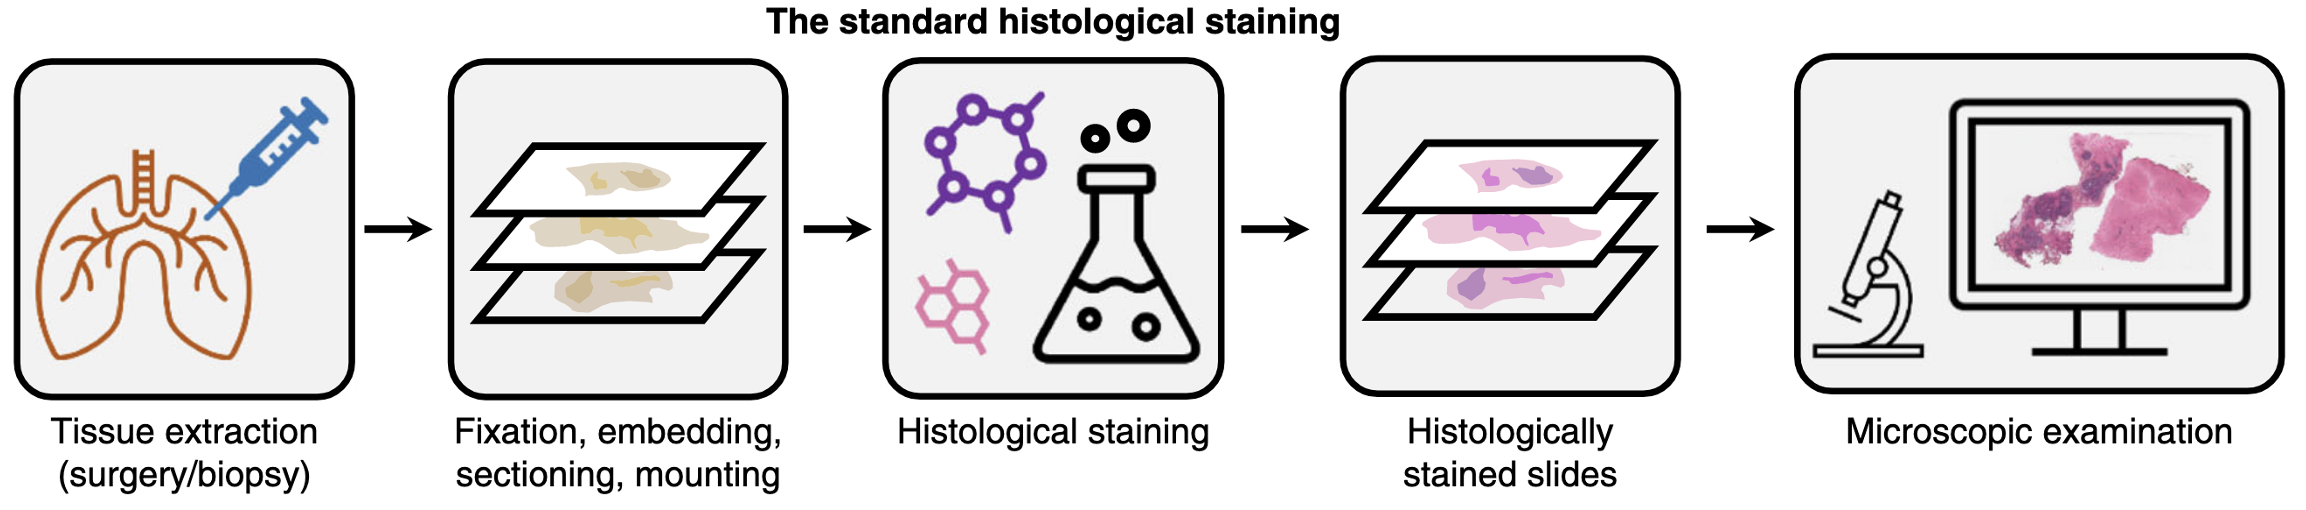
\includegraphics[width=1\textwidth]{Images/Histology_Summary.png}
  \caption{From \cite{bai_deep_2023}}
  \label{fig:hist-summary}
\end{figure}

New methods are being developed to expedite the cancer diagnosis process by using machine learning in conjunction with a range of imaging technologies including stimulated Raman spectroscopy (SRS) \cite{hollon_near_2020, sarri_fast_2019, kondepudi_foundation_2024, jiang_opensrh_2022}, second harmonic generation microscopy (SHG) \cite{sarri_fast_2019}, and Fourier transform infrared spectroscopy (FTIR) \cite{tomas_detection_2022, berisha_deep_2019}. The This project will focus on ........
\subsection{Future Vision}
\subsection{Novelty of This Work}